% -*- root: ../thesis.tex -*-
%!TEX root = ../thesis.tex
% ******************************* Thesis Chapter 8 ****************************


% ----------------------- paths to graphics ------------------------

% change according to folder and file names
\graphicspath{{8/figures/}}
% ----------------------- contents from here ------------------------

Since no comparable framework exists, it is hard to compare this software to others.
The evaluation should therefore determine to which degree the outputs of the Hawk framework can be integrated and if all requirements, as specified in the requirements section, are fulfilled. This evaluation focuses on the DLP input abstraction and the new Hawk module, as this thesis added them. 

\section{Hawk DLP}
\begin{figure}[!h]
  \centering

  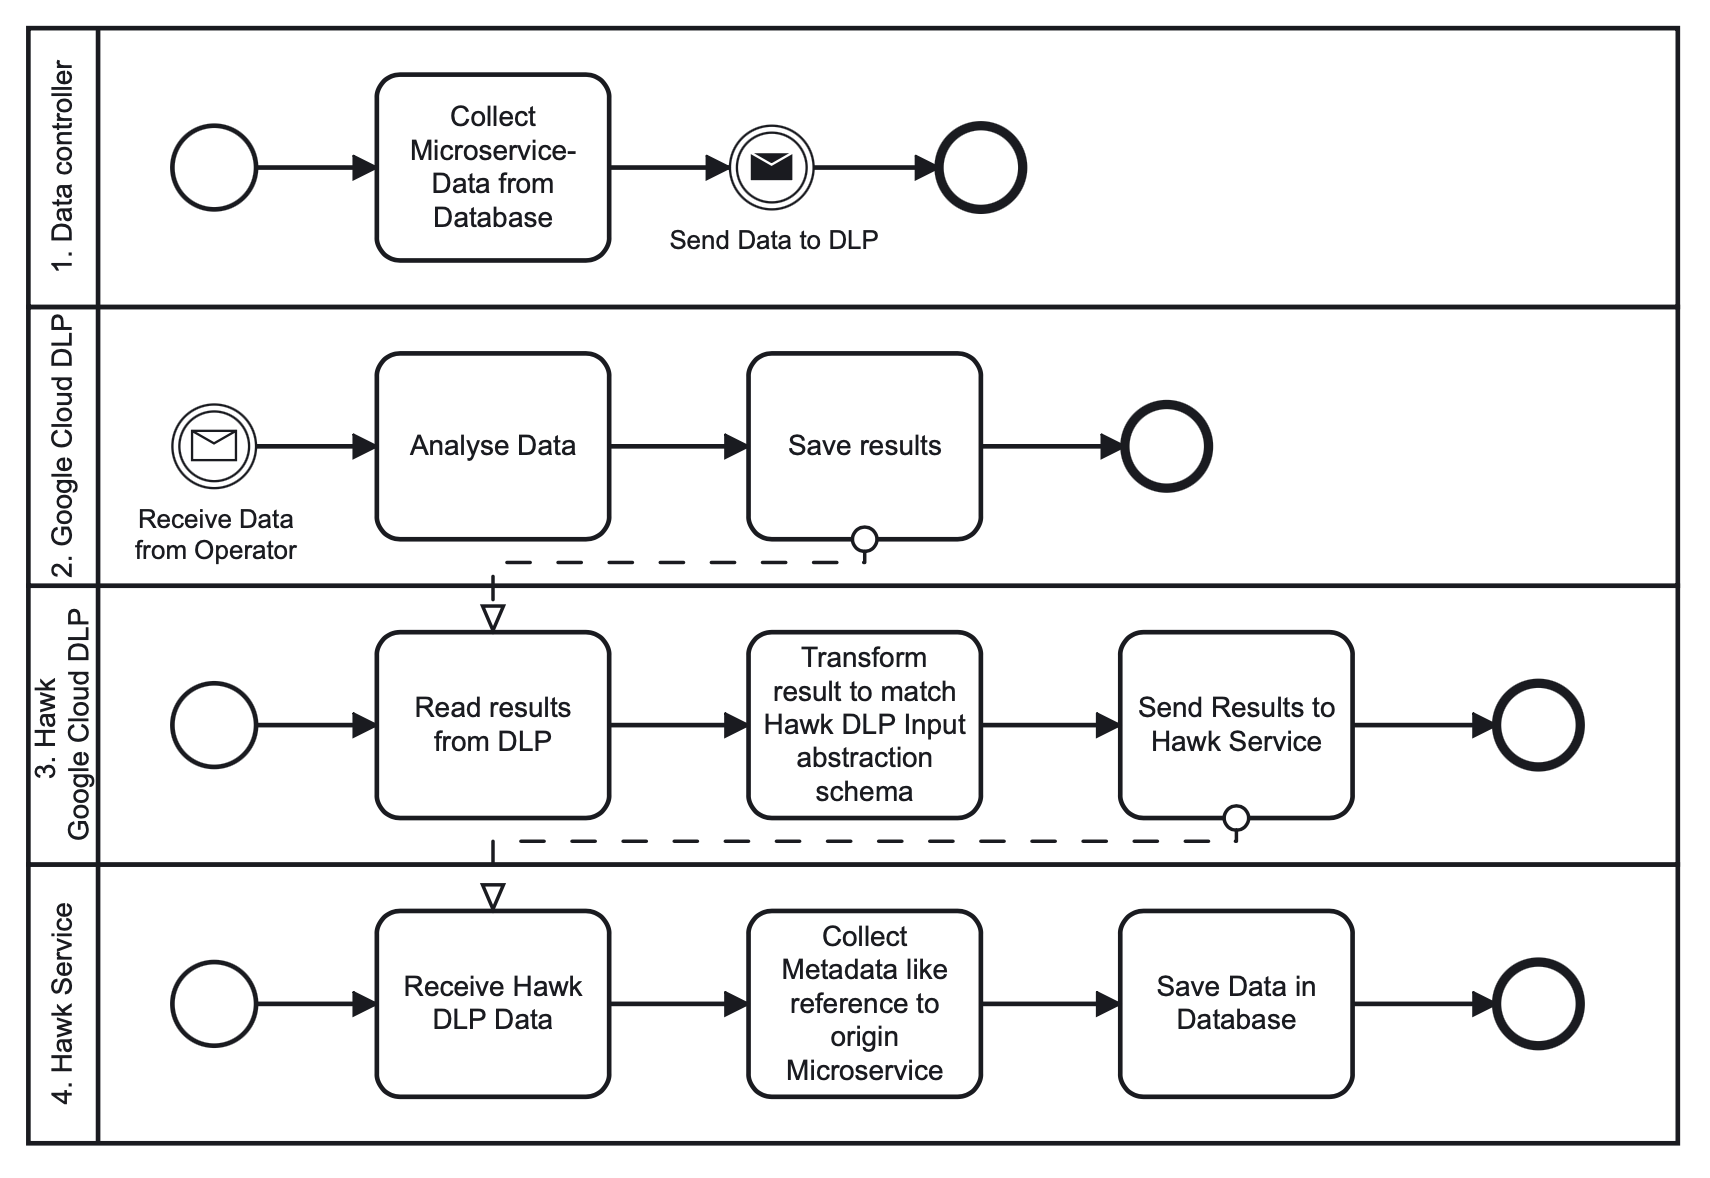
\includegraphics[width=0.95\columnwidth]{bpmn.png}

  \caption[Hawk exemplary DLP process]{An exemplary process of how the Data loss prevention integration backed by Google Cloud DLP works using the Hawk framework.}  
  \label{fig:hawk-dlp-uml}
\end{figure}

Figure \ref{fig:bpmn} shows how the evaluation of the Hawk framework will be done. An exemplary microservice application will be used as a data source here. In the first step of the figure, dumps of the databases will be taken and sent to the chosen DLP technology over the API provided by the respective DLP Input. In the next step, the DLP will process the data externally. When finished, the respective Hawk DLP input will read the results with the vendor-specific API. The third step processes these results and sends them to the Hawk service. In the fourth step, inside the Hawk service, the results get annotated with all the information from the Hawk modules. The annotated results will then be saved in a database and are accessible via. the Hawk API.

\section{AWS Macie vs. Google Cloud DLP}
As mentioned in the sections above, AWS Macie only offers one way to inspect data. The Macie DLP input there submits a \texttt{ClassificationJob}, which will be asynchronously processed. With some tests made, this took on average around 13 minutes, which might be because of the scheduling on the part of AWS. Note that changing the size in the number of 10s of rows of the CSV submitted did not change the processing time in any meaningful way. As seen in the demonstration video, available in the Hawk DLP GitHub project.


Google CDLP offers two ways of inspecting data, where one is synchronous and directly returns the results found, and the other is asynchronous similar to AWS. However, the latter could be implemented yet, because results are published to a BigQuery table rather than being available via REST API. Since the effort needed to implement this was too big for this thesis, it is hard to compare both Jobs directly. For this reason, the synchronous endpoint was used, which took around 200ms on average for Google to respond. As seen in the demonstration video, available in the Hawk DLP GitHub project.

% ---------------------------------------------------------------------------
%: ----------------------- end of thesis sub-document ------------------------
% ---------------------------------------------------------------------------